\newcommand{\kernel}{\mathsf{Ker}}
\newcommand{\Id}{\mathsf{Id}}


\section{Separation of Matrix Parameterizations}

Given $C = \{C_i\}_{i \in [n]} \subset \R^{k \times k}$, define the cone 
\[ K_C = \{ x \in \R^n \mid \sum_{i \in [n]}  C_i x_i \succeq 0\}   \]
Here $C$ is said to be a spectrahedral representation of the cone $K_C$.

\begin{definition}
	A spectrahedral representation of a cone $K  \subseteq \R^n$ as $K = \{ x \in \R^n | \sum_i C_i x_i \succeq 0\}$,is said to be a {\it normalized} if,
    	\[ \sum_{i = 1}^n C_i = \Id_k \]
        and $C_i \succeq 0$
 \end{definition}
 
 \begin{lemma} \label{lem:normalization}
	If a spectrahedral cone $K$ contains the positive orthant $\R_{+}^n$ then $K$ admits a normalized representation.
 \end{lemma}

 \begin{proof}
Let $C = \{C_i\}_{i \in [n]}$ be a spectrahedral representation of $K$.
%
Let $U = \cap_{i = 1}^n \kernel(C_i)$ be the subspace in the kernel of all the $C_i$, and let $\Pi_{U^\perp}$ denote the projection on to $U^{\perp}$.  It is easy to check that for all $x \in \R^n$,
 \[ \sum_i C_i x_i \succeq 0 \iff \sum_i \Pi_{U^{\perp}} C_i \Pi_{U^{\perp}} x_i \succeq 0 .\]
 By a basis change of $\R^n$, that contains a basis for $U^{\perp}$, we obtain matrices $C' = \{C'_i\}_{i \in [n]}$ in $\R^{k' \times k'}$ where $k' = \dim(U^{\perp})$ such that $K = K_{C'}$.
 
Furthermore, since the $i^{th}$ basis vector $e_i$ is in the non-negative orthant, $e_i \in K$.  This implies that $C'_i \succeq 0$ for each $i$.  For each $u \in U^{\perp}$, there exists $C_i$ such that $u^T C_i u > 0$, which implies that 
$\sum_i u^T  C'_i u > 0$.  In other words, we have $M = \sum_i C'_i \succ 0$ is positive definite.

The normalized representation of $K$ is given by $C'' = \{ M^{-1/2}C'_i M^{-1/2}\}_{i \in [n]}$.  By definition, the representation is normalized in that $\sum_{i \in [n]} C''_i = \Id_{k'}$.
 \end{proof}
 
For two spectrahedral representations given by matrices $ C = \{C_i\}_{i \in [n]} $ and $C' = \{C'_i\}_{i \in [n]}$, define the distance between the representations as,
\[ \mdist(C, C')  = \max_i \| C_i - C'_i \| \]

\begin{lemma} \label{lem:conetomatrices}
Suppose $C, C'$ are normalized spectrahedral representations of $K_C$ and $K_{C'}$ respectively.  Then,
$\hdist(K_C, K_{C'}) \leq n^{3/2} \cdot \mdist(C,C')$
\end{lemma}
\begin{figure}
	\centering
	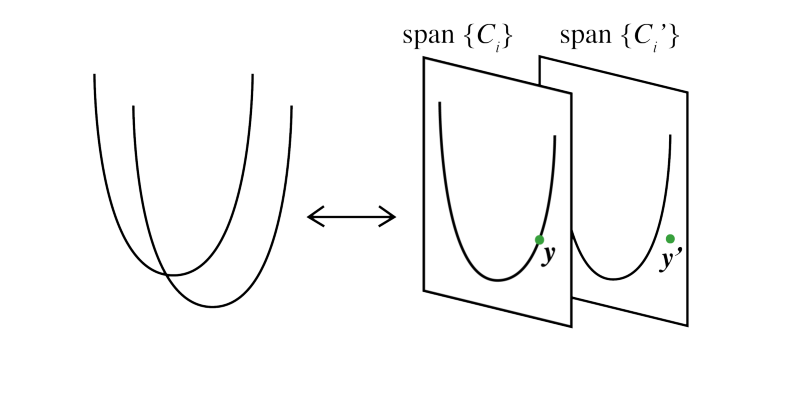
\includegraphics[width=0.6\textwidth]{sections.PNG}
	\caption{Proof of Lemma \ref{lem:conetomatrices}}
\end{figure}

\begin{proof}
Let $B(0,1)$ denote the $\ell_\infty$ unit ball in $\R^n$.  For every $x \in K_C \cap B(0,1)$, 
\begin{align*}
 \sum_{i \in [n]} C'_i x_i & = \sum_{i \in [n]} C_i x_i + \sum_{i \in [n]} (C_i-C'_i) x_i \\
 & \succeq - n \mdist(C,C') \cdot \Id_k 
 \end{align*}
where we are using the fact that $\sum_i C_i x_i \succeq 0$.  This implies that the point $x' =  x + n \mdist(C,C') \cdot \one \in K_{C'}$.  To see this, recall that the representation is normalized in that $\sum_i C'_i = \Id_k$.  Therefore, we get 
\[ \sum_i C'_i x'_i = \sum_i C'_i x_i + n \cdot \mdist(C,C') \sum_i C'_i \succeq 0 \]
The lemma follows by observing that $\|x - x'\|_2 \leq n^{3/2} \cdot \mdist(C,C')$.

\end{proof}
